\documentclass[10pt,a4paper]{article}
\usepackage[utf8]{inputenc}
\usepackage{amsmath}
\usepackage{amsfonts}
\usepackage{amssymb}
\usepackage{graphicx}
\usepackage{url}
%
\usepackage[a4paper,bindingoffset=0.2in,left=1in,right=1in,top=1in,bottom=1in,footskip=.25in]{geometry}
%
\title{The HERA RFI environment}
\author{Saul A. Kohn\thanks{saulkohn@sas.upenn.edu; University of Pennsylvania}}


\begin{document}
\maketitle

\abstract{In this memo I describe the RFI properties of the HERA site, as recorded by PAPER-128 during it's most recent observation season.}

\section{Introduction}

The PAPER-128 2014 observation season ran from 18th June 2014 through the 30th April 2015. During this run, some 200 nights of data were recorded. A ``night", which I will refer to using the JD at the start of observations, consists of twelve hours of observation from 6pm to 6am South African Standard Time (SAST). Observations as processed by the PAPER/HERA correlator are recorded in {\sc miriad} ``uv" files. These files contain visibilities for each antenna pair in the array. Each integration is 20 seconds long over 1024 frequency bins from 100 to 200\,MHz. Each uv file contains 56 integrations per antenna pair, and  280 uv files are recorded per linear polarization (xx, xy, yx, yy) per night.


Early in the PAPER data compression process, visibilities are flagged for radio frequency interference (RFI). This is accomplished by the {\sc aipy} script \textit{xrfi\_simple.py}, which takes the derivative of the frequency axis of all baselines associated with antenna 1 (2nd row, 4th column of the redundant grid), and flags any frequencies with a derivative $\geqslant 6\sigma$ above the mean. We always flag the band-edges ($\sim$7\,MHz on each side), since these frequencies are not useful to us, and always flag the 137$\pm$0.6\,MHz band associated with ORBCOMM satellite network transmissions. This process is repeated per integration within each uv file and stored in a {\sc python} npz file. This means that any baseline associated with antenna 1 can contribute a flag to the resultant npz file, which in turn is applied to the data. The result is 280 files of high-time and -frequency resolution files per night per linear polarization containing information about the low-frequency RFI environment of he HERA site. In this memo I report on the properties of these flags in time- and frequency-space over the 2014 observation season.

XXX explain ``threshold=80"

XXX not really wording it well yet

XXX talk about narrow vs broadband RFI

XXX talk about why we care?

\section{Average Properties}

In order to assess the average properties of the HERA RFI environment, I calculated a weighted average of flags over the season. Over 200 nights, one-time occurrences are washed-out beneath the 1\% level, allowing me to assess persistent issues without much distraction. 

Nominally, each night should grant 3920 integrations-worth of flags over 1024 frequency bins, per linear polarization. In reality, most of the time this holds true, but occasionally not all files are compressible (hence failing to generate flags) or observations fail to start at the correct time (so there are no data to flag upon). Also, in the event of an X-engine failure within the correlator, contiguous chunks of the band (in eighths, i.e. 25\,MHz across) are flagged-out, usually for the rest of the night.

For this reason, I calculated a weighted average of the flags across the season, but neglected nights with correlator failures or late starts. Weights were simply the number of nights that contained that integration-bin in SAST. The resultant ``average waterfall" is shown in Figure~\ref{fig:average-waterfall}. The color scale is indicative of flagging frequency across the season, and line plots above and to the right of the the waterfall showing the percentage of times and frequencies that were flagged, respectively. 

A summary of the persistent (flagged $\geq1\%$ of the time per channel) RFI frequencies can be found in Table~\ref{tab:main}. I have investigated each frequency and tried to find the most likely source for each. In most cases, this required looking at the properties in time as well as frequency. Others were more obvious from frequency alone, e.g. the 149.8\, MHz transmission frequency from the ISS. Still others I could not track down a convincing explanation for, and these are listed with a `?'. A `?' next to a possible cause indicates that the listed cause is the most prevalent at that frequency, but that the temporal properties of that cause do not necessarily make sense. 

\begin{figure}
\centering
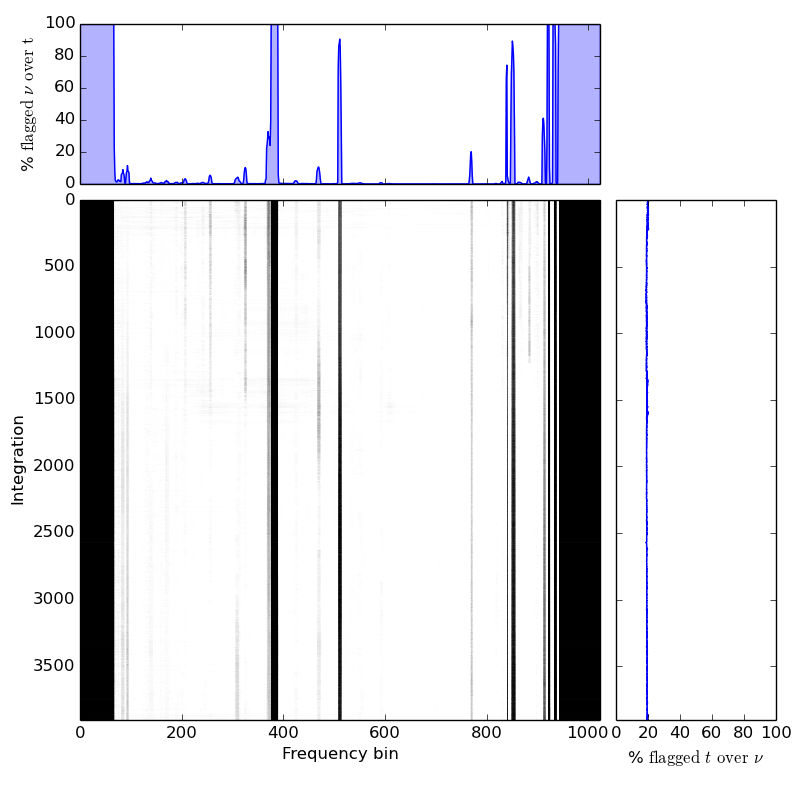
\includegraphics[width=\textwidth]{RFI-images/149days.png} %149 days including day 0 = 150 days... my bad...
\caption{A waterfall plot of RFI flags averaged over 150 days of data. The gridding process is described in the text. Above the waterfall I show the percentage of the season each frequency is flagged, and to the right I show the percentage of frequencies that are flagged per integration. XXX remake this plot with time in hours and frequency in MHz}
\label{fig:average-waterfall}
\end{figure}

\begin{table}
\centering
\small
\caption{RFI frequencies and brief characterization (if possible) for the averaged-down flags}
\begin{tabular}{llll}
\hline
$\nu$ 	&	flagged 	&	Cause	&	Notes/	\\
(MHz) & (\%) & (Possible) &SAST Characterization\\
\hline
103	$\pm$	3	&	100	&	BAND EDGE	&		\\
107.25	$\pm$	0.25	&	2.6	&	FM radio	&	Constant background at 2\% level	\\
107.55	$\pm$	0.05	&	1.9	&	FM radio	&	Constant background at 2\% level	\\
108.1	$\pm$	0.4	&	9	&	FM radio?	&	Rises with time, peaking at midnight and 4am	\\
109	$\pm$	0.4	&	11.5	&	FM radio?	&	Rises with time, peaking around 4am	\\
112.8	$\pm$	0.1	&	1.4	&	Aircraft?	&	Constant background at 1\% level	\\
114.05	$\pm$	0.85	&	3.7	&	?1	&	Decreases till midnight; peak at 4am	\\
116.55	$\pm$	0.35	&	2.2	&	?2	&	Peak at midnight	\\
120.15	$\pm$	0.35	&	3.2	&	Aircraft	&	Roughly follows CPT$\leftrightarrow$JNB flight times	\\
124.95	$\pm$	0.35	&	5.5	&	Aircraft	&	Roughly follows CPT$\leftrightarrow$JNB flight times	\\
130.25	$\pm$	0.55	&	4.3	&	?3	&	Falls (7pm) and rises (3am) steeply 	\\
131.75	$\pm$	0.35	&	10.3	&	Aircraft?	&	Peaks at 6:30, 7:30, 8:30, 9:30, 10 and then a steep falloff	\\
136.05	$\pm$	0.45	&	33.1	&	Radar?	&	Decreases over night	\\
137.35	$\pm$	0.85	&	100	&	ORBCOMM	&		\\
141.45	$\pm$	0.35	&	2.1	&	Mobile phones?	&	High until 9pm, then at background 1\% level	\\
145.85	$\pm$	0.45	&	10.7	&	Amateur radio& Strong 9pm-1am -- this is the official downlink for ISS-HAM	\\
149.75	$\pm$	0.55	&	90.7	&	ISS	&	``Beeps", but in stacked data peaks 2am	\\
175.15	$\pm$	0.35	&	20.5	&	VHF TV	 (video) &	 Channel 4. Peaks at 8:30pm, then falls to background 7\%	\\
181.15	$\pm$	0.15	&	1.6	&	VHF TV (audio) & Channel 4. 2\% level turns-off at 10pm	\\
182.15	$\pm$	0.35	&	75	&	?4	&	Decreases until 10pm (to ~15\%), when it begins a slow rise again	\\
183.2	$\pm$	0.5	&	89.7	&	VHF TV (video)	&	Channel 5. Rises throughout night. 	\\
186.25	$\pm$	0.35	&	4.6	&	?5	&	Extreme turn-off at 9:45	\\
189.15	$\pm$	0.35	&	41.4	&	VHF TV (audio)	&	Channel 5. Rises throughout night. 	\\
189.9	$\pm$	0.4	&	100	&	BAND?	&	\\
191.1	$\pm$	0.3	&	100	&	BAND?	&	\\
196	$\pm$	4	&	100	&	BAND EDGE	&	\\
\hline
\end{tabular}
XXX find out why David flags the 190 and 191 MHz bands
\label{tab:main}
\end{table}

\subsection{Characterization}

Table~\ref{tab:main} provides a brief characterization of each frequency in SAST. In this subsection I elaborate on these characterizations. Many of the characterizations arise from the South African Table of Frequency Allocations (SATFA; \cite{SAFreqTable}).

Figure~\ref{fig:freqflags} shows the detail of the top panel of Figure~\ref{fig:average-waterfall}. This figure highlights the broad swath of the band from roughly 150 to 180\,MHz that is completely clear of RFI. This roughly corresponds to 21\,cm redshifts $z=6.9$ to 8.5 -- and this is one of the reasons that the \cite{Parsons.14} and \cite{Ali.15} limits on the 21\,cm power spectrum concentrated on this redshift range -- there are simply more unflagged data to average-down with. \cite{Furlanetto.06} show that the $z\sim8$ universe can be considered roughly coeval over an $\sim$8\,MHz bandwidth. As such, the 30\,MHz chunk(XXX) could be used to create $\sim$3 power spectra, as demonstrated in \cite{Jacobs.15}.

\begin{figure}
\centering
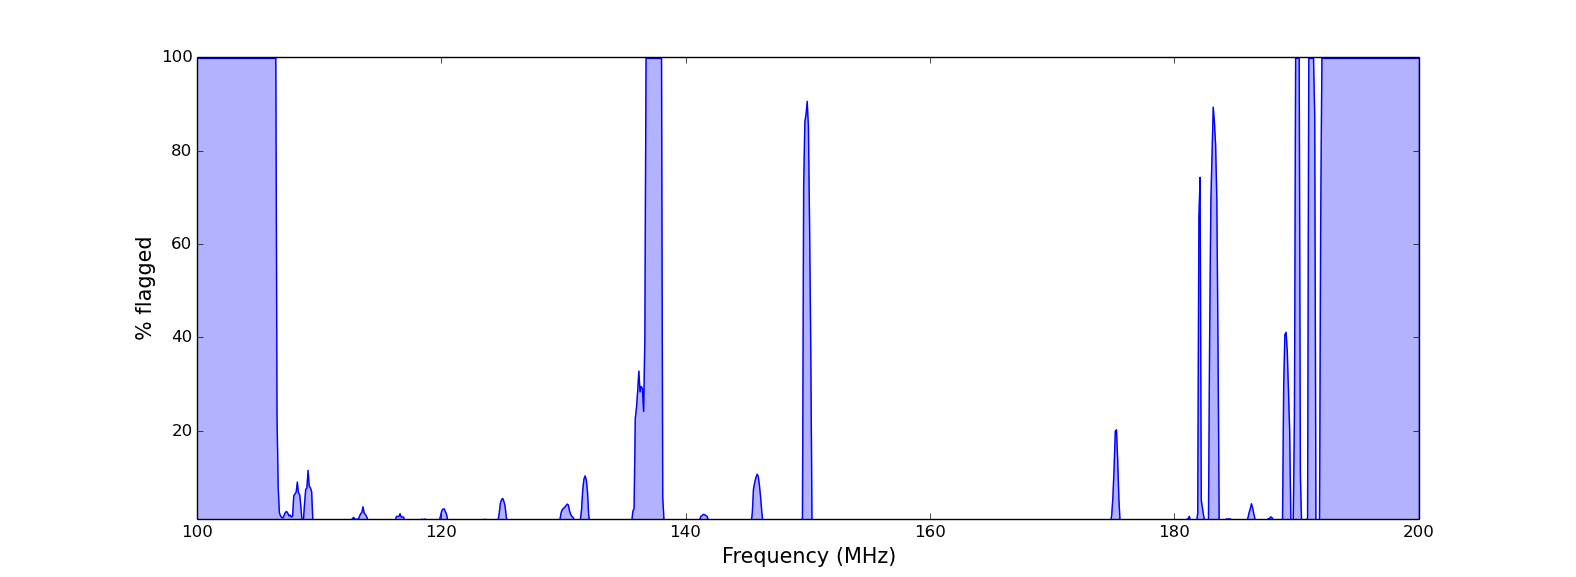
\includegraphics[width=\textwidth]{RFI-images/149days-freq.png}
\caption{The percentage of time that each frequency was flagged over the season.}
\label{fig:freqflags}
\end{figure}

\subsubsection{FM radio}

SATFA lists the frequency band 87.5--108\,MHz as available for FM radio broadcasts, leading me to postulate that the low-level RFI we observe in the 107.25	$\pm$	0.25 and 107.55	$\pm$	0.05\,MHz bands has FM radio as the leading cause. The 108.1	$\pm$	0.4 and 109	$\pm$	0.4\,MHz bands are outside of the official range, and exhibit odd temporal properties for human activity -- two peaks at midnight and 4am with a increasing number of flags throughout the average night (see Figure~\ref{fig:FMradio}). 

\begin{figure}
\centering
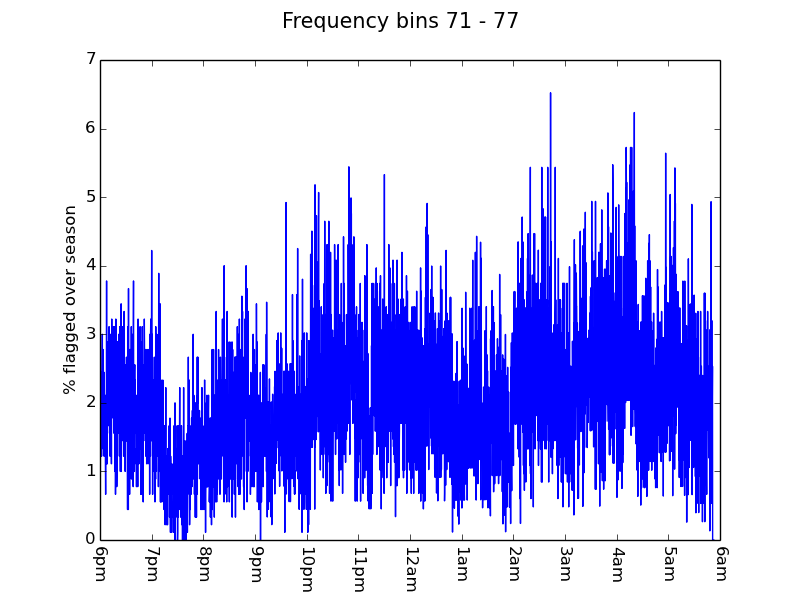
\includegraphics[width=0.4\textwidth]{RFI-images/FB_71_77.png}
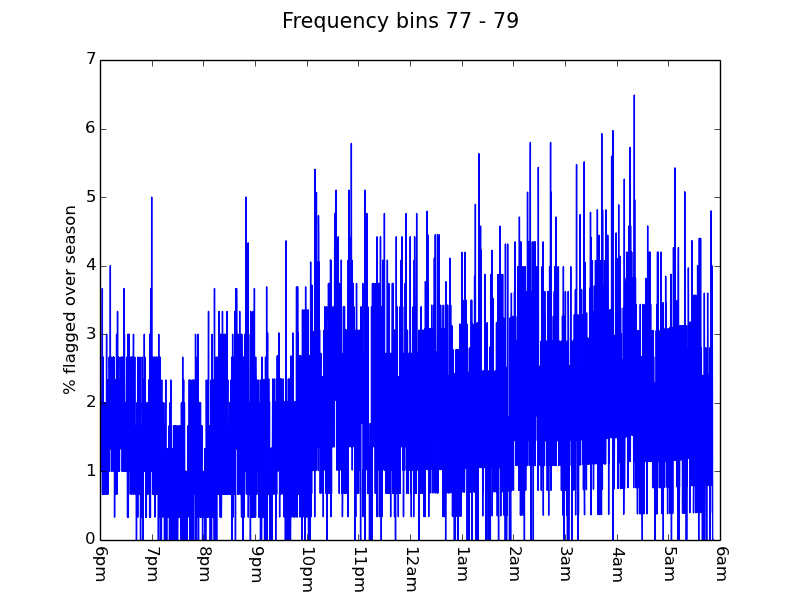
\includegraphics[width=0.4\textwidth]{RFI-images/FB_77_79.png}
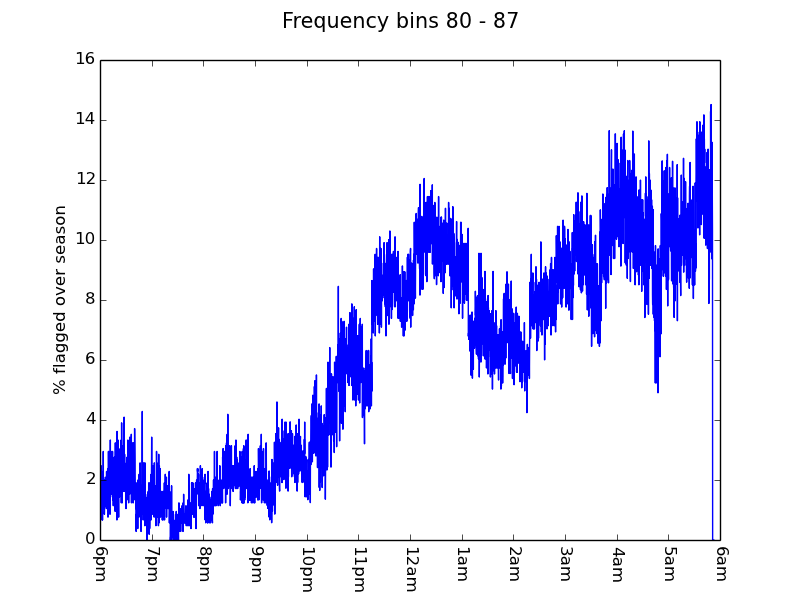
\includegraphics[width=0.4\textwidth]{RFI-images/FB_80_87.png}
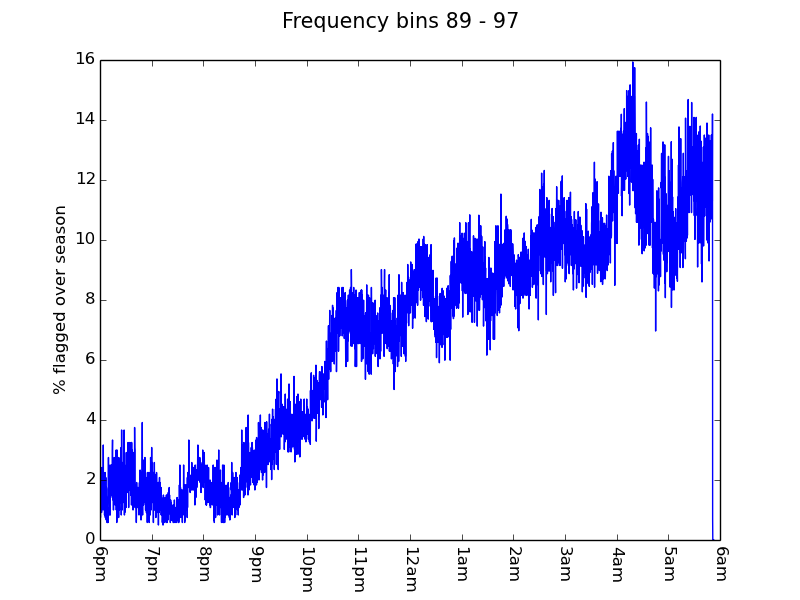
\includegraphics[width=0.4\textwidth]{RFI-images/FB_89_97.png}
\caption{Possible FM radio contamination in the \textit{Top, left to right}: 107.25$\pm$0.25 and 107.55$\pm$0.05\,MHz bands, and \textit{Bottom, left to right}: 108.1$\pm$0.4 and 109$\pm$0.4\,MHz bands.}
\label{fig:FMradio}
\end{figure}

\subsubsection{Aircraft communications}

It is difficult to argue that the 112.1$\pm$0.1\,MHz signal is caused by aircraft communications since it maintains a constant background level. However, SATFA lists this frequency as reserved for aircraft communications and it has been used in the past as a calibration frequency for aircraft instruments \cite{AircraftCalibrationFreqs}.

The other aircraft frequencies are obvious, because they closely trace the 2-hour flight from Cape Town to Johannesburg\footnote{Credit to Danny Jacobs for first spotting this and noting it in an internal PAPER circular in December 2009.}. 
An example (120.15$\pm$0.35\,MHz) is shown in Figure~\ref{fig:aircraft}. SATFA reserves frequencies 108--117.975\,MHz for aeronautical radionavigation and 117.975--137\,MHz for aeronautical mobile. In Table~\ref{tab:main} I list 131.75$\pm$0.35\,MHz as caused by aircraft since it falls in the aeronautical mobile band, but it does not follow the flight patterns as closely as the other bands.

\begin{figure}
\centering
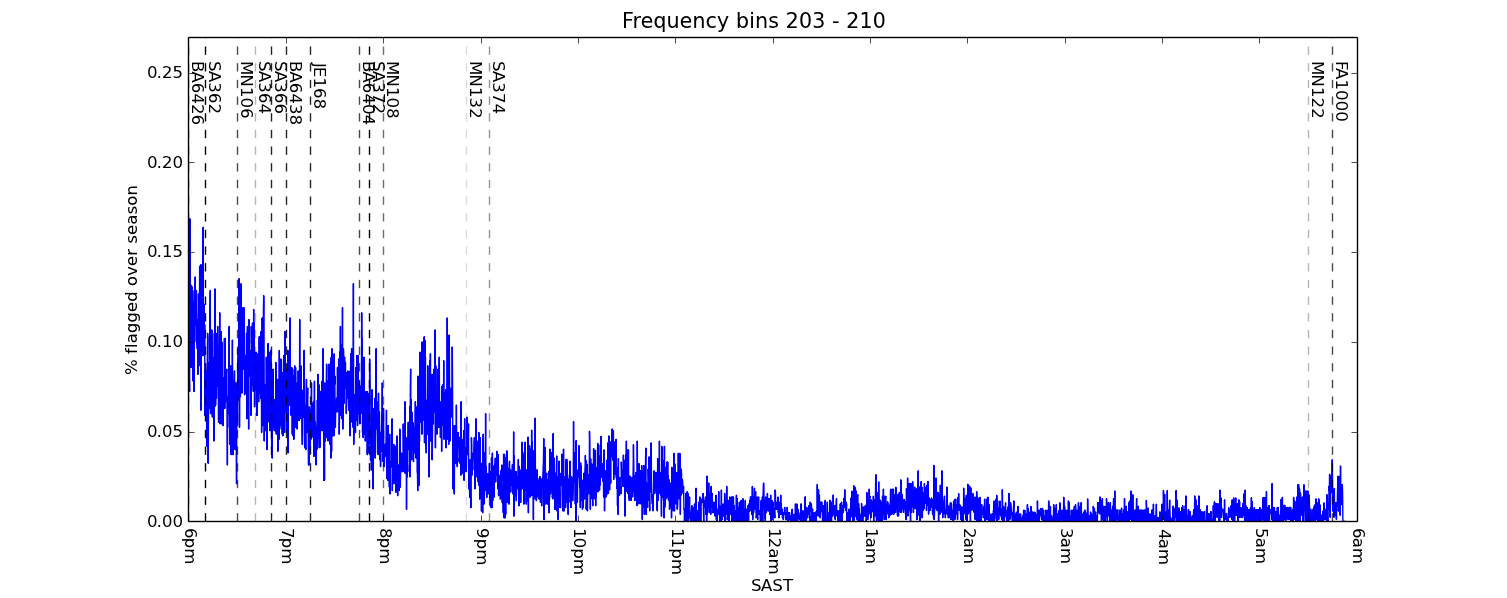
\includegraphics[width=\textwidth]{RFI-images/aircraft_chan_203-210.png}
\caption{
XXX FIX THE Y-AXIS
Flights from Cape Town to Johannesburg correspond to RFI in the 120.15$\pm$0.35\,MHz channels. Vertical dashed lines indicate a flight leaving Cape Town (flights from Johannesburg are roughly concurrent) and the flight code is listed. The transparency of a line is inversely proportional to how many days a week that flight is scheduled for. The flight is 2 to 2.5 hours long -- and about 2 hours after the last flight of the day, the flags fall to background level (but notably, not always to zero).}
\label{fig:aircraft}
\end{figure} 

\subsubsection{Orbital communications}
The \textit{Global Frequency Database}\footnote{\url{http://qrg.globaltuners.com/}} (GFD) lists an (unconfirmed) AM signal at 134.4\,MHz with callsign `RADAR' in  North-East Johannesburg\footnote{There is an active HAM radio operator/survivalist in South Africa with a hobby for what he refers to as `rapid deployment of amateur radio stations (RaDAR)'. He might be the origin of this callsign. It could be worth getting in touch with him and letting him know that he may be interfering with our science. See \url{https://zs6bne.wordpress.com/}.}. This may be the source of the 136.05$\pm$0.45\,MHz signal present in 1/3\,rd of the season	. It could also be `spillage' of signal from ORBCOMM. 

ORBCOMM Inc.'s constellation of 29 LEO communication satellites is a well-known contaminant of the low-frequency sky, dominating over any astronomical signal at 137--138\,MHz (although each satellite emits within a 20\,kHz band). For this reason we have built flags at 137.35$\pm$0.85\,MHz into the compression pipeline.

The largest contaminant without flags built-in to the pipeline is communications from the International Space Station (ISS). The 149.75$\pm$0.55\,MHz transmissions are semi-regular in time; they `beep'.  

Onboard the ISS are HAM radio devices. Some countries have also launched satellites with these onboard, one of the purposes of which is to provide HAM radio operators something in space to communicate with. These devices are licensed to operate at 145.2 and 145.8\,MHz, and SATFA lists the whole 144-146\,MHz band as reserved for `Amateur--Satellite' communications. We detect RFI at 145.85$\pm$0.45\,MHz, although strong signal across $\sim$10\% of the season that occurs 9pm-1am argues against human operation. 

\subsubsection{Mobile phones and VHF TV}

A weak RFI signal at 141.45$\pm$0.35\,MHz is within the `mobile 1 BTX'  and aeronautical mobile band in SATFA, but other than this listing I do not have a strong case for the signal.

The strong signals at 183.2$\pm$0.5\,MHz and 189.15$\pm$	0.35\,MHz have almost identical gradients for the percentage of flagging as a function of time of night. These frequencies correspond exactly to Channel 5 of South African System I 625-line VHF TV signals for video and audio transmission, respectively. Similarly, the weaker signals at 175.15$\pm$0.35	 and 181.15$\pm$0.15\,MHz correspond to Channel 4's video and audio transmission, respectively, but they do not share the same temporal properties. Still, VHF TV is the best bet given the matching video/audio frequencies.

\subsubsection{Unidentified sources}

There are 5 RFI frequencies in the averaged data that I cannot identify the sources of:  weak emissions (flagged $<5\%$ of the season) at 114.05$\pm$0.85, 116.55$\pm$0.35, 130.25$\pm$0.55 and 186.25$\pm$0.35\,MHz, and one strong emission at 182.15$\pm$0.35\,MHz. The variation of each source with time is shown in Figure~\ref{fig:unidentified}. The 186.25$\pm$0.35\,MHz has a sharp turn-off around 9:45pm each night, suggesting that it is some kind of automated device.

\begin{figure}
\centering
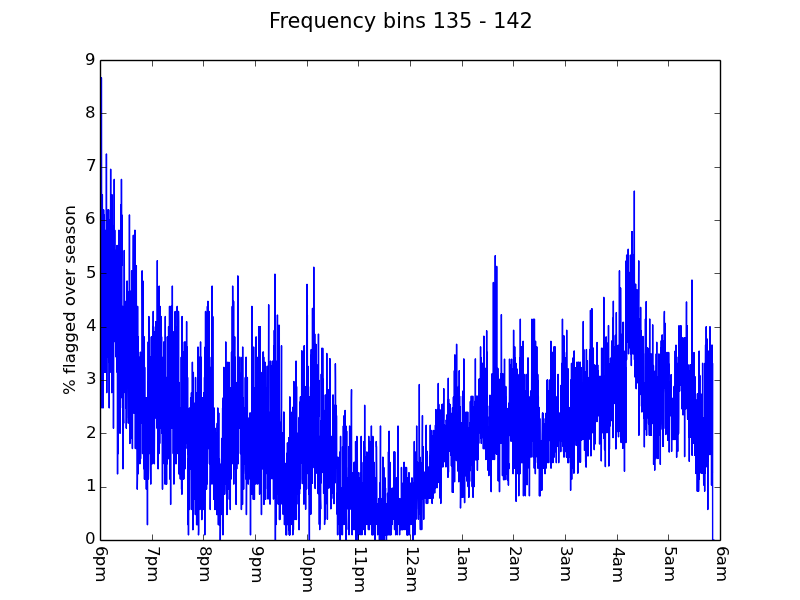
\includegraphics[width=0.4\textwidth]{RFI-images/FB_135_142.png}
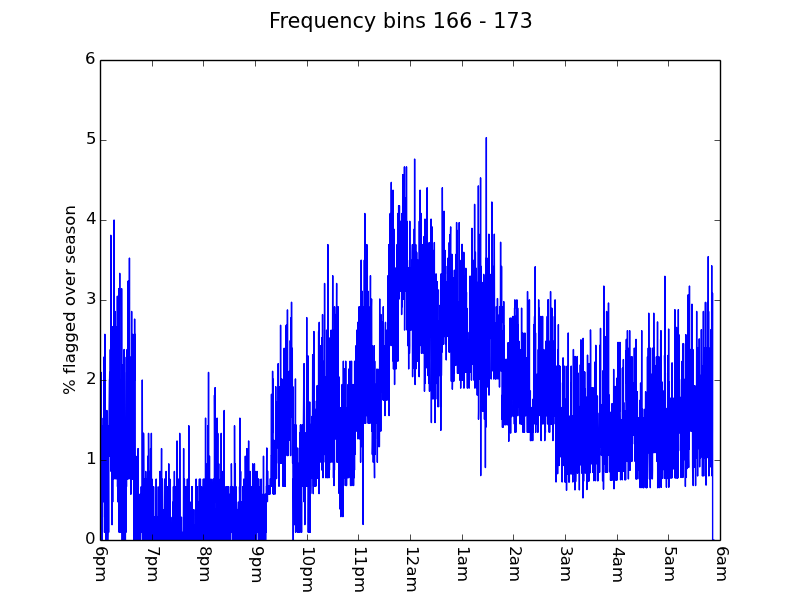
\includegraphics[width=0.4\textwidth]{RFI-images/FB_166_173.png}
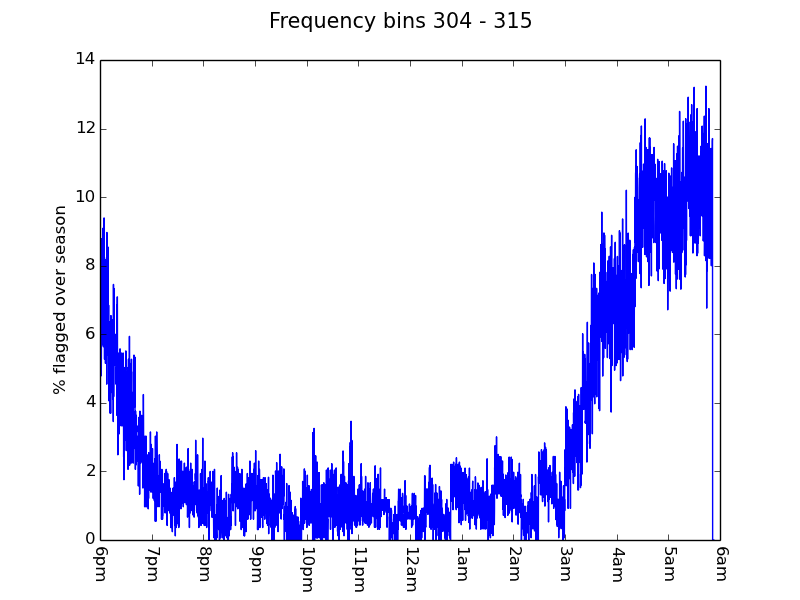
\includegraphics[width=0.4\textwidth]{RFI-images/FB_304_315.png}
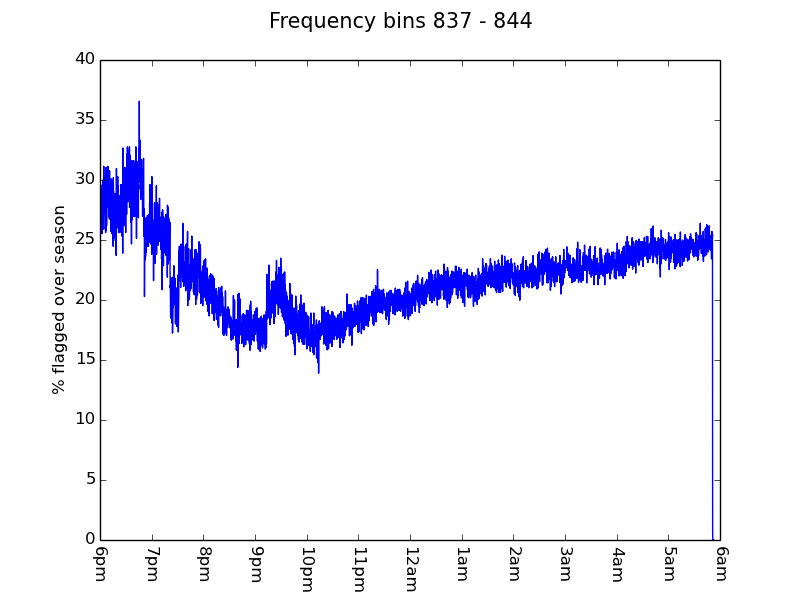
\includegraphics[width=0.4\textwidth]{RFI-images/FB_837_844.png}
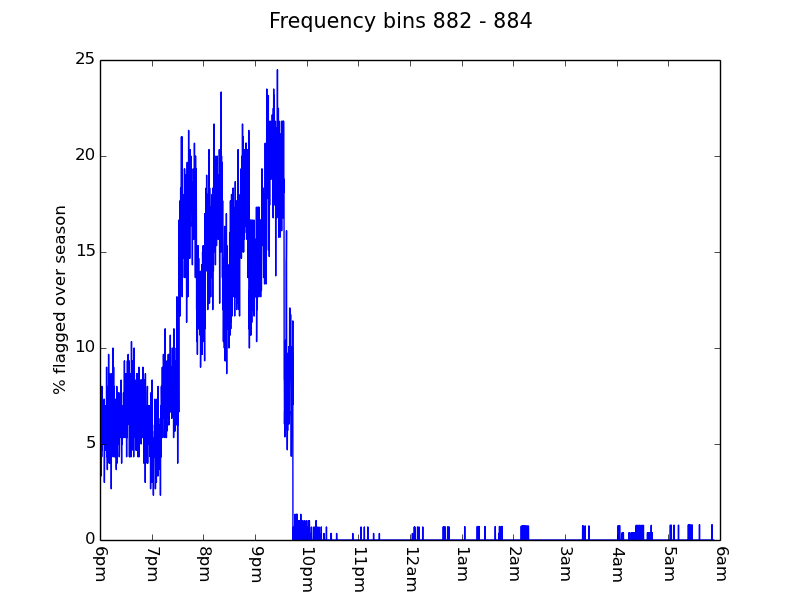
\includegraphics[width=0.4\textwidth]{RFI-images/FB_882_884.png}
\caption{The temporal profile of the 5 RFI frequencies with unidentified causes. \textit{Top, left to right:} 114.05$\pm$0.85 and 116.55$\pm$0.35\,MHz. \textit{Middle, left to right:} 130.25$\pm$0.55 and 182.15$\pm$0.35\,MHz. \textit{Bottom:} 186.25$\pm$0.35\,MHz. The 182.15$\pm$0.35\,MHz frequency is flagged a large amount of the time, making it our most-offending unidentified source.}
\label{fig:unidentified}
\end{figure}


\section{Individual Properties}

The previous section addresses season-long problems with RFI. In this section I discuss the properties of individual nights.

Using the flags per night, I was able to take a look at the total number of flags as a percentage of the waterfall (i.e. $N_{\rm flags}/(3920\times1024)$). The average flagging per night is 19.2\% (XXX HOW MUCH DO PERMANENT FLAGS CONTRIBUTE), with a standard deviation of 0.5\%. Four nights deviate from the average by $\geq 2\sigma$ (in the `more flags' direction; there are no deviations this large in the `fewer flags' direction): JDs 2456965, 2456732, 2456958 and 2457038. Their flag waterfalls are shown in Figure~\ref{fig:worst} (2456732, 2456958 and 2457038) and Figure~\ref{fig:wandering} (2456965). While the strange nature of night 2456965 is discussed below, the three others follow the pattern of having strong contamination from FM and aircraft communication bands, but also have broadband `pulses' up to about 20mins in length. The source of these broadband pulses is not well understood, and very troubling XXX EXPAND.

\begin{figure}
\centering
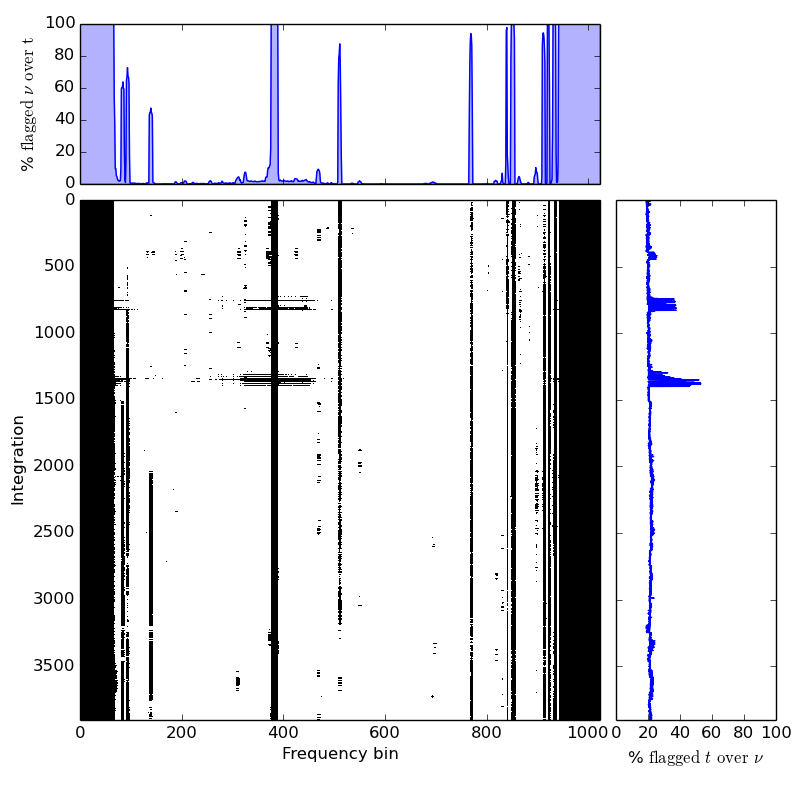
\includegraphics[width=0.3\textwidth]{RFI-images/2456732RFI.png}
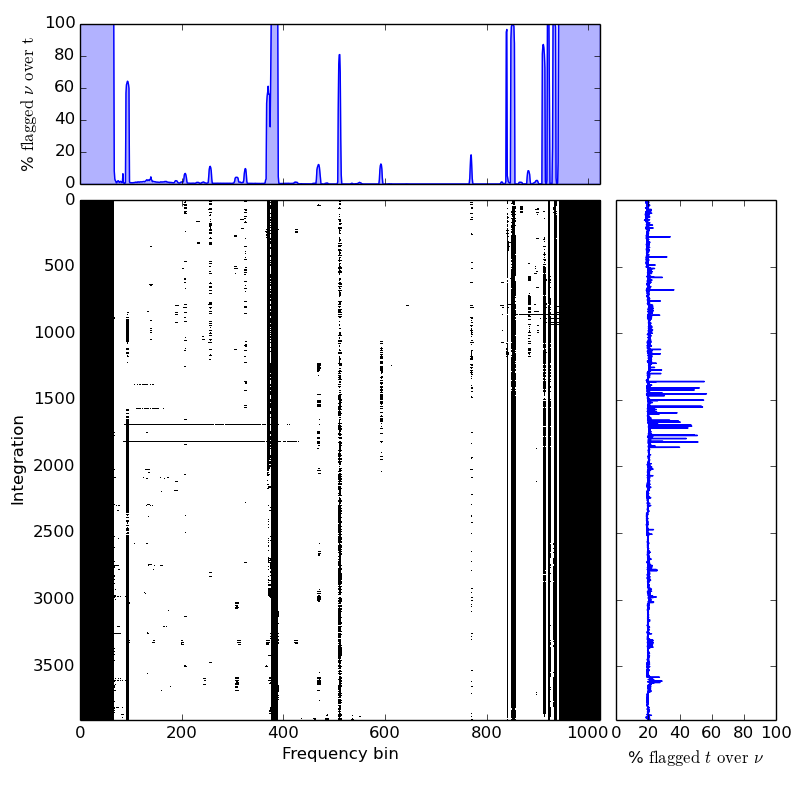
\includegraphics[width=0.3\textwidth]{RFI-images/2456958RFI.png}
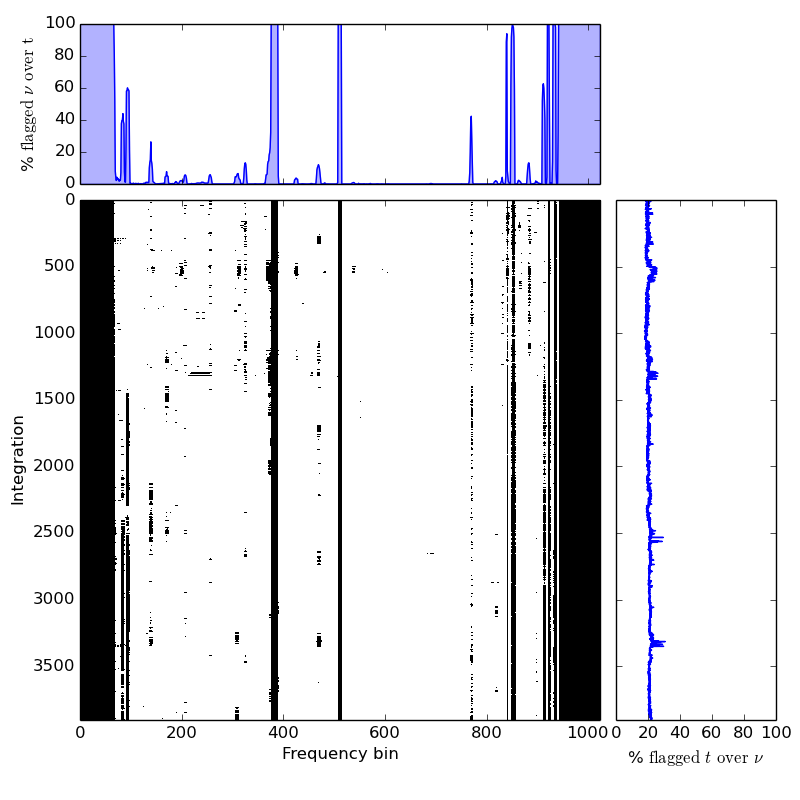
\includegraphics[width=0.3\textwidth]{RFI-images/2457038RFI.png}
\caption{\textit{Left to right:} waterfalls of flags for nights 2456732, 2456958 and 2457038. These three nights, along with 2456965, are $>$20.2\% flagged; $>2\sigma$ above the average flagging amount per night.}
\end{figure}


JD 2456965 is easily the worst offender, and it exhibits a strange signal that wanders in frequency and time close to the ISS band. An event of note on this date (23rd November 2014) was a Soyuz FG launch that docked with the ISS -- could this signal be a signature of their transmissions\footnote{The internet also suggests... less plausible explanations: \url{https://www.youtube.com/watch?t=11&v=VtZx8iPO4zs}. }? 
Similar signals are seen on 2456898 (28th August 2014; although only at the beginning of the night) and 2456924 (23rd September 2014). There is no listed orbital or suborbital activity for 2456898. There was an US ICBM test off of the coast of Virginia on 2456924, but this is probably not the cause of the RFI.
The flag waterfalls for these nights are shown in Figure~\ref{fig:wandering}.

\begin{figure}
\centering
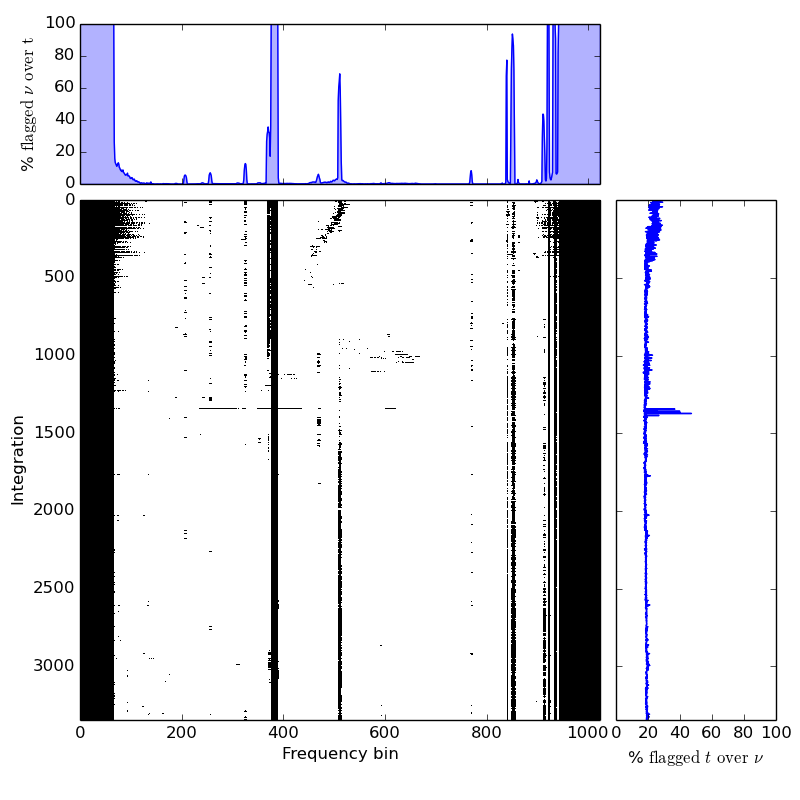
\includegraphics[width=0.3\textwidth]{RFI-images/2456898RFI.png}
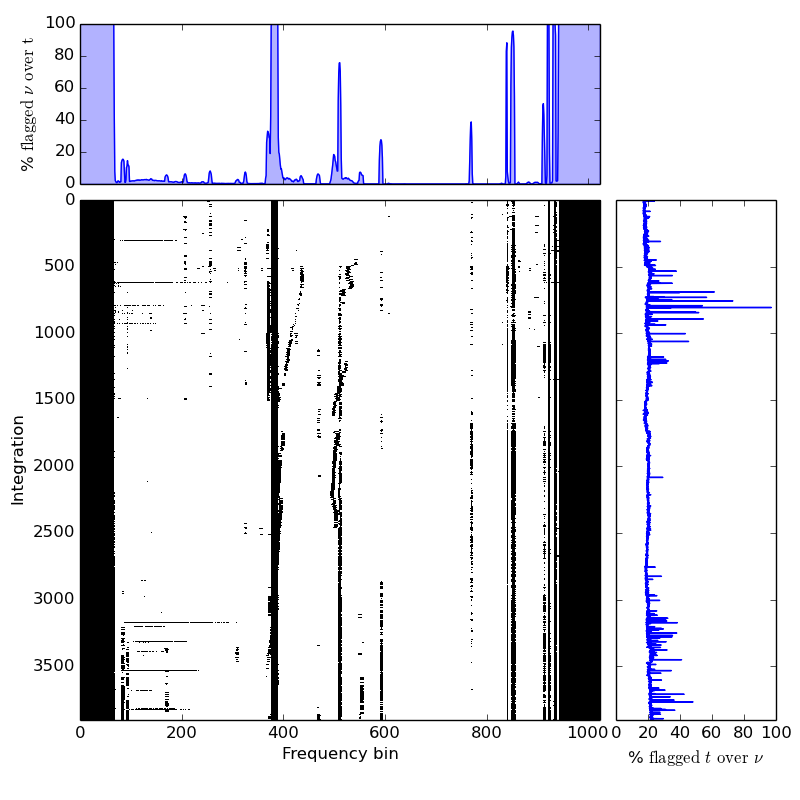
\includegraphics[width=0.3\textwidth]{RFI-images/2456924RFI.png}
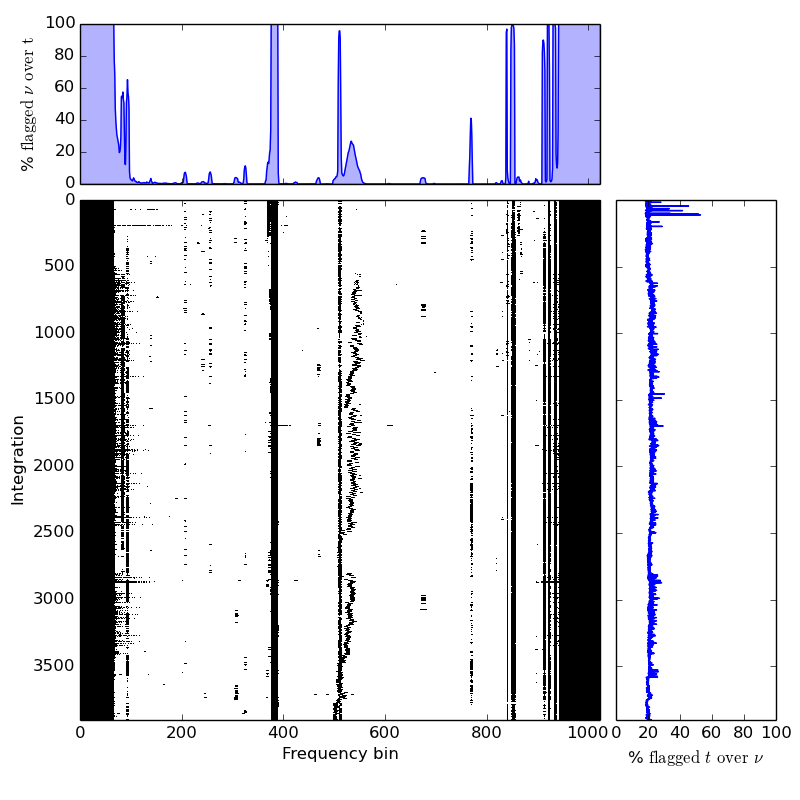
\includegraphics[width=0.3\textwidth]{RFI-images/2456965RFI.png}
\caption{\textit{Left to right:} waterfalls of flags for nights 2456898, 2456924 and 2456965. These three nights exhibit a strange behaviour of RFI that changes in frequency and time. JD 2456965 is by far the worst, and during this night as well as 2456898, we see a broadband `comb' of flagged frequencies near the band edges}
\label{fig:wandering}
\end{figure}

\section{Conclusions}

What does all this mean for HERA? I feel like I have left more questions than answers in this memo. However, there are some actions that can be taken:
\begin{itemize}
\item Certain parties that the HERA collaboration is in contact with have the authority to shut-down VHF TV signals in the SKA radio-quiet zone. Steps should be taken towards disabling Channel 4 and Channel 5 transmissions in the area, since these are clearly interfering with our measurements.
\item The ISS 149.75$\pm$0.55\,MHz band should be permanently flagged within the compression pipeline along with ORBCOMM and the band edges.
\item XXX say something about broadband RFI
\item XXX  anything else?
\end{itemize}

I should note that after compression, our frequency resolution decreases dramatically. If a low-resolution frequency bin contains a frequency that has been flagged at the high-resolution flagging stage, the low-resolution bin is also flagged. This caveat means that analyses that work with HERA data in its compressed form (i.e. DDR-filtering) as opposed to a higher frequency resolution stage (i.e. FHD) will have different views of the amount of RFI in a given visibility. 

Meanwhile, a new, lower-frequency feed is currently under development by the HERA analog group. This would nominally allow measurements to be taken in the range 50--250\,MHz, allowing science observations of the Dark Ages and the post-reionization Universe. While an XXXawesome science objective, it should be noted that at the lowest frequencies FM radio will be a constant harassment to these measurements. At the higher frequencies, VHF TV will be the primary contaminant, but should be much easier to remove as it is both narrow-band and, as noted above, shut-down-able.

XXX get bibliography unfucked

\bibliographystyle{plain}
\bibliography{RFImemoBib}


\end{document}